\chapter{Arhitektura i dizajn sustava} \label{arhitektura}
		
%		\textbf{\textit{dio 1. revizije}}\\
		
%		\textit{ Potrebno je opisati stil arhitekture te identificirati: podsustave, preslikavanje na radnu platformu, spremišta podataka, mrežne protokole, globalni upravljački tok i sklopovsko-programske zahtjeve. Po točkama razraditi i popratiti odgovarajućim skicama:}

%	\begin{itemize}
%		\item 	\textit{izbor arhitekture temeljem principa oblikovanja pokazanih na predavanjima (objasniti zašto ste baš odabrali takvu arhitekturu)}
%		\item 	\textit{organizaciju sustava s najviše razine apstrakcije (npr. klijent-poslužitelj, baza podataka, datotečni sustav, grafičko sučelje)}
%		\item 	\textit{organizaciju aplikacije (npr. slojevi frontend i backend, MVC arhitektura) }		
%	\end{itemize}



%   OVDJE PIŠE ŠTO TREBA NAPISATI!---^^^
		
    \noindent { Arhitektura se može podijeliti na tri podsustava:}
	\begin{itemize}
		\item{Web poslužitelj}
		\item{Web aplikacija}
		\item{Baza podataka}		
	\end{itemize}
	
	\underline{\textit{Web poslužitelj}} osnova je rada web aplikacije. Njegova primarna zadaća je komunikacija klijenta s aplikacijom. Komunikacija se odvija preko HTTP (engl. Hyper Text Transfer Protocol) protokola, što je protokol u prijenosu informacija na webu. Poslužitelj je onaj koji pokreće web aplikaciju te joj prosljeđuje zahtjev.
	
	Korisnik koristi \underline{\textit{web aplikaciju}} za obrađivanje željenih zahtijeva. Web aplikacija obrađuje zahtjev te ovisno o zahtjevu, pristupa bazi podataka, vraća web-poslužitelju odgovor u JSON formatu, a zatim web poslužitelj te informacije prikazuje na svoj način.
		\begin{figure}[H]
                    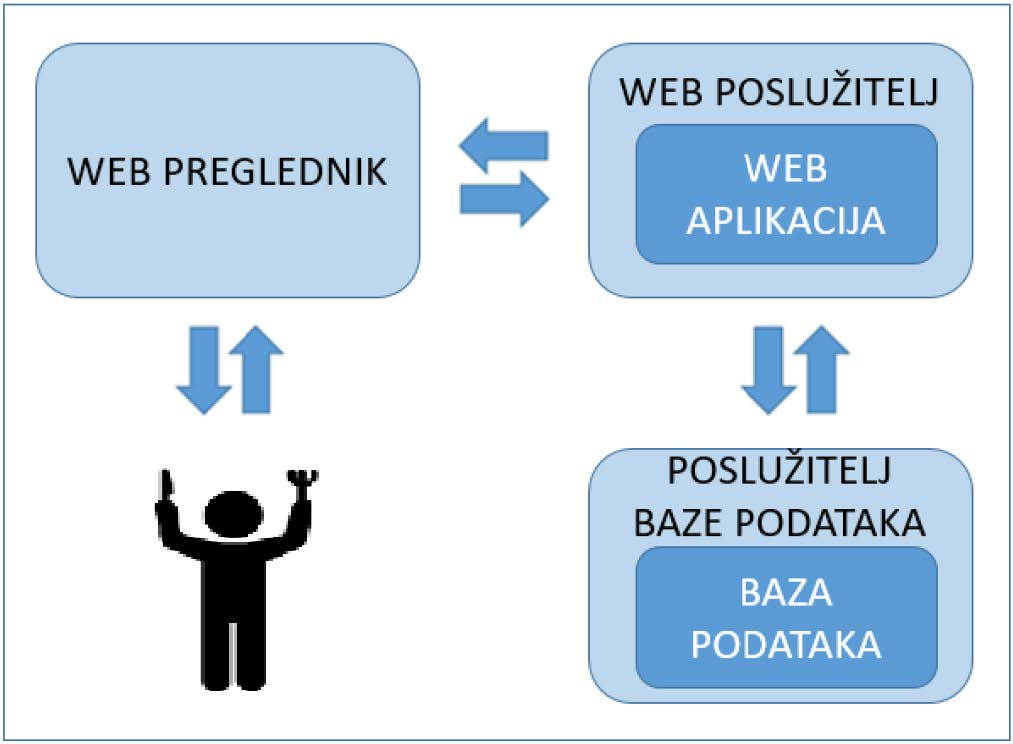
\includegraphics[scale=1]{slike/Arhitektura sustava.jpg}
        			\centering
        			\caption{Arhitektura sustava}
        			\label{fig:hztm-stranica}
        		\end{figure}
			
			\eject

	Programski jezik koji smo odabrali za izradu naše web aplikacije je Java zajedno sa SpringBoot radnim okvirom te programski jezik Javascript s React bibliotekom (eng. library). Odabrano razvojno okruženje je IntelliJ. 
	
	Arhitektura sustava sastoji se od 3 razine:
	\begin{itemize}
		\item{\textbf{Sučelje} - Najviša razina aplikacije, glavna funkcija sučelja je prevesti procese i rezultate u format koji korisnik može razumijeti}
		\item{\textbf{Logika} - Ova razina koordinira aplikaciju, obrađuje naredbe, izvršava logiku i računa. Također prenosi podatke između podatkovne razine i sučelja.}
		\item{\textbf{Podatci} - Ova razina uključuje spremanje i dohvaćanje podatke iz baze podataka}		
	\end{itemize}
	
	Funkcionalnosti aplikacije se izvršavaju slanjem upita na \textit{\underline{endpointe}}. Oni definiraju adresu ili točku spajanja na Web poslužitelj. Tipično je reprezentiran jednostavnim HTTP URL-om (adresom, \textit{linkom}).
	
	Implementirani Endpointi su:
	\begin{itemize}
	    \item {\textbf{Prijava} - Omogućava pristup korisničkom računu, provjerava jeli dobro postavljen session cookie}
	    \item {\textbf{Kreiranje donora od strane donora}}
	    \item {\textbf{Kreiranje donora od strane radnika}}
	    \item {\textbf{Prikaz korisničkih podataka}}
	\end{itemize}

	

	
		

		

				
		\section{Baza podataka}
			
%			\textbf{\textit{dio 1. revizije}}\\
			
		Sustav koristi relacijsku bazu podataka. Relacijske baze podataka pohranjuju i pružaju pristup podatcima. Gradivna jedinka baze je relacija, odnosno tablica koja je definirana svojim imenom i skupom atributa. Prednost relacijskih baza jest lakše definiranje odnosa između podataka. Baza podataka ove aplikacije sastoji se od ovih entiteta:
		\begin{itemize}
	        \item Korisnik
	        
	        \begin{itemize}
	            \item Donor krvi
	            \item Djelatnik banke
	        \end{itemize}
	        
	        \item Zaliha krvi
	        \item Pokušaj donacije
	        
	        
	    \end{itemize}
		
		
			\subsection{Opis tablica}
			

		%		\textit{Svaku tablicu je potrebno opisati po zadanom predlošku. Lijevo se nalazi točno ime varijable u bazi podataka, u sredini se nalazi tip podataka, a desno se nalazi opis varijable. Svjetlo zelenom bojom označen je primarni ključ. Svjetlo plavom označen je strani ključ. Svijetlo tirkiznom bojom označen je ključ koji je primarni i strani. Svijetlo crvenom bojom označeni su unique atributi koji nisu ključevi.}
				
				
				
				
			% OVO STAVI KAO NASLOV SVAKE TABLICE U OVE PRVE UGLATE ZAGRADE, GDJE PIŠE LABEL=NONE (mozes vidjeti primjer kod dnevnika promjena)
			%caption = {Dnevnik promjena dokumentacije}
			
		\textbf{Korisnik} - Ovaj entitet sadržava sve administrativne podatke o korisniku aplikacije, njegovi osnovni podatci nalaze se u drugim, personiliziranim entitetima. Sadrži atribute: user id, user role, password, acc activated, perm deactivated, opt out. Ovaj entitet u vezi je \textit{One-to-one} sa entitetima Donorom i Djelatnikom banke preko atributa donor id, odnosno bank worker id. 
			
				\begin{longtblr}[
				    caption = {Tablica \textit{korisnik} u bazi podataka},
					label=none
					]{
						width = \textwidth,
						colspec={|X[6,l]|X[7, l]|X[20, l]|}, 
						rowhead = 1,
					} %definicija širine tablice, širine stupaca, poravnanje i broja redaka naslova tablice
					\hline \multicolumn{3}{|c|}{\textbf{Korisnik}}	 \\ \hline[3pt]
					\SetCell{LightGreen}user id & BIGINT	&  	Jedinstveni identifikator korisnika  	\\ \hline
					user role	& VARCHAR(20) &  Je li korisnik donor, djelatnik  banke ili administrator 	\\ \hline 
					password & VARCHAR(128) &  Enkriptirana lozinka korisnika \\ \hline 
					acc activated & INT	& Je li korisnik preko e-maila aktivirao svoj račun  		\\ \hline 
					perm deactivated & INT &  Je li korisnički račun trajno dekativiran \\ \hline 
					opt out & INT &  Je li uključena opcija koja isključuje notifikacije \\ \hline 
				\end{longtblr}
				
				
		\textbf{Donor} - Ovaj entitet sadržava osobne podatke o korisniku aplikacije koji je donor. Sadrži atribute: donor id, first name, last name, oib, birth date, birth place, address, work place, private contact, work contact, email, blood type. Ovaj entitet u vezi je \textit{One-to-many} sa entitetom Pokušaj donacije preko atributa donor id. Također je u vezi \textit{One-to-one} sa entitetom Korisnik preko atributa donor id.
				
				\begin{longtblr}[
				    caption = {Tablica \textit{donor} u bazi podataka},
					label=none
					]{
						width = \textwidth,
						colspec={|X[6,l]|X[7, l]|X[20, l]|}, 
						rowhead = 1,
					} %definicija širine tablice, širine stupaca, poravnanje i broja redaka naslova tablice
					\hline \multicolumn{3}{|c|}{\textbf{Donor}}	 \\ \hline[3pt]
					\SetCell{LightTeal}donor id & BIGINT	&  	Jedinstveni identifikator donora krvi, odgovara identifikatoru korisnika  	\\ \hline
					first name	& VARCHAR(50) &  Ime donora krvi 	\\ \hline 
					last name & VARCHAR(50) &  Prezime donora krvi \\ \hline 
					\SetCell{LightRed}oib & CHAR(11)	& OIB donora krvi  		\\ \hline 
					birth date & DATE &  Datum rođenja donora krvi \\ \hline 
					birth place & VARCHAR(100) &  Mjesto rođenja donora krvi \\ \hline 
					address & VARCHAR(100)	& Adresa stanovanja donora krvi  		\\ \hline 
					work place & VARCHAR(100) &  Mjesto zaposlenja donora krvi \\ \hline 
					private contact & VARCHAR(20) &  Osobni kontakt broj mobitela donora krvi \\ \hline 
					work contact & VARCHAR(20) &  Poslovni kontakt broj mobitela donora krvi \\ \hline 
					email & VARCHAR(50) &  e-mail adresa donora krvi \\ \hline 
					\SetCell{LightBlue}blood type & VARCHAR(3) &  Krvna grupa donora krvi \\ \hline 
					perm rejected reason & VARCHAR(100) &  Ako je račun donora krvi trajno deaktiviran, razlog deaktivacije \\ \hline
				\end{longtblr}
				
		\textbf{Djelatnik banke} - Ovaj entitet sadržava osobne podatke djelatnika banke. Sadrži atribute: bank worker id, first name, last name, oib, birth date, birth place, address, work place, private contact, work contact, email. U vezi je \textit{One-to-one} sa entitetom Korisnik preko atributa bank worker id.
				
				\begin{longtblr}[
				    caption = {Tablica \textit{djelatnik banke} u bazi podataka},
					label=none
					]{
						width = \textwidth,
						colspec={|X[6,l]|X[7, l]|X[20, l]|}, 
						rowhead = 1,
					} %definicija širine tablice, širine stupaca, poravnanje i broja redaka naslova tablice
					\hline \multicolumn{3}{|c|}{\textbf{Djelatnik banke}}	 \\ \hline[3pt]
					\SetCell{LightTeal}bank worker id & BIGINT	&  	Jedinstveni identifikator djelatnika banke, odgovara identifikatoru korisnika  	\\ \hline
					first name	& VARCHAR(50) &  Ime djelatnika banke  	\\ \hline 
					last name & VARCHAR(50) &  Prezime djelatnika banke  \\ \hline 
					\SetCell{LightRed}oib & CHAR(11)	& OIB djelatnika banke   		\\ \hline 
					birth date & DATE &  Datum rođenja djelatnika banke  \\ \hline 
					birth place & VARCHAR(100) &  Mjesto rođenja djelatnika banke  \\ \hline 
					address & VARCHAR(100)	& Adresa stanovanja djelatnika banke  		\\ \hline 
					work place & VARCHAR(100) &  Mjesto zaposlenja djelatnika banke  \\ \hline 
					private contact & VARCHAR(20) &  Osobni kontakt broj mobitela djelatnika banke  \\ \hline
					work contact & VARCHAR(20) &  Poslovni kontakt broj mobitela djelatnika banke  \\ \hline 
					email & VARCHAR(50) &  e-mail adresa djelatnika banke  \\ \hline 
				\end{longtblr}
				
		\textbf{Zaliha krvi} - Ovaj entitet sadržava podatke o količini krvi u banci. Sadrži atribute: number of units, max units, min units.
			
				\begin{longtblr}[
				    caption = {Tablica \textit{zaliha krvi} u bazi podataka},
					label=none
					]{
						width = \textwidth,
						colspec={|X[6,l]|X[6, l]|X[20, l]|}, 
						rowhead = 1,
					} %definicija širine tablice, širine stupaca, poravnanje i broja redaka naslova tablice
					\hline \multicolumn{3}{|c|}{\textbf{Zaliha krvi}}	 \\ \hline[3pt]
					\SetCell{LightGreen}blood type & CHAR(3) & Krvna grupa jedinice krvi \\ \hline
					number of units	& INT &  Trenutni broj jedinica krvi  	\\ \hline 
					max units & INT &  Maksimalni broj jedinica krvi \\ \hline 
					min units & INT	& Minimalni broj jedinica krvi \\ \hline 
				\end{longtblr}
				
		\textbf{Pokušaj donacije} - Ovaj entitet sadržava podatke o pojedinoj donaciji krvi. Sadrži atribute: donation id, rejected reason, blood type, donor id, bank worker id. U vezi je \textit{Many-to-one} sa entitetom Donor preko atributa donor id.
		        
				\begin{longtblr}[
				    caption = {Tablica \textit{pokušaj donacije} u bazi podataka},
					label=none
					]{
						width = \textwidth,
						colspec={|X[6,l]|X[7, l]|X[20, l]|}, 
						rowhead = 1,
					} %definicija širine tablice, širine stupaca, poravnanje i broja redaka naslova tablice
					\hline \multicolumn{3}{|c|}{\textbf{Pokušaj donacije}}	 \\ \hline[3pt]
					rejected reason	& VARCHAR(100) &  Razlog neuspješnosti pokušaja darivanja krvi 	\\ \hline 
					\SetCell{LightBlue}blood type & CHAR(3) &  Kvrna grupa donora krvi koji obavlja ovu donaciju \\ \hline 
					\SetCell{LightBlue}donor id & BIGINT	& Jedinstveni identifikator donora krvi koji obavlja ovu donaciju krvi \\ \hline 
					\SetCell{LightBlue}bank worker id & BIGINT	& Jedinstveni identifikator djelatnika banke koji nadgleda ovu donaciju krvi \\ \hline 
				\end{longtblr}
				
				
			
			\subsection{Dijagram baze podataka}
			
				
				\begin{figure}[H]
                    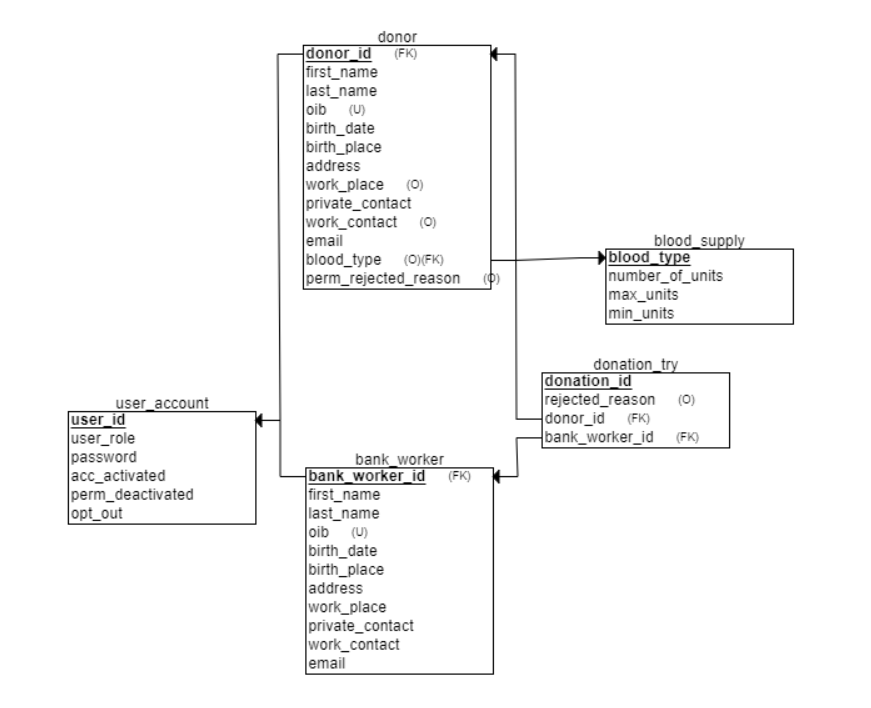
\includegraphics[scale=0.9]{slike/relational schema.png}
        			\centering
        			\caption{Relacijska shema baze podataka}
        			\label{fig:hztm-stranica}
        		\end{figure}
			
			\eject
			
			
		\section{Dijagram razreda}
		
%			\textit{Potrebno je priložiti dijagram razreda s pripadajućim opisom. Zbog preglednosti je moguće dijagram razlomiti na više njih, ali moraju biti grupirani prema sličnim razinama apstrakcije i srodnim funkcionalnostima.}\\
			
%			\textbf{\textit{dio 1. revizije}}\\
			
%			\textit{Prilikom prve predaje projekta, potrebno je priložiti potpuno razrađen dijagram razreda vezan uz \textbf{generičku funkcionalnost} sustava. Ostale funkcionalnosti trebaju biti idejno razrađene u dijagramu sa sljedećim komponentama: nazivi razreda, nazivi metoda i vrste pristupa metodama (npr. javni, zaštićeni), nazivi atributa razreda, veze i odnosi između razreda.}\\

Na slikama u nastavku prikazani su razredi koji pripadaju "backend" dijelu arhitekture. Slike su podlijeljene po pripadnosti odgovarajćim entitetima iz baze podataka koji su opisani u poglavlju 4.1 (Baza podataka). Za svaki entitet postoje klase sljedećih tipova:
\begin{itemize}
	        \item \textbf{Controller} - Vraća "response entity" objekt koji sadrži http status i .json objekt na endpoint-e. Obično se radi o vraćanju podataka iz baze podataka. Controller također određuje korisničke dozvole pristupa pojedinim endpoint-ima  .
	        \item \textbf{Service} - Obavlja poslovnu logiku aplikacije. To uključuje validaciju računa, kreiranje računa, provjeru podataka itd.
	        \item \textbf{Repository} - Vadi i sprema podatke iz baze podataka, koristeći Spring Data JPA.
	        \item \textbf{Model} - Objekt koji je mapiran na entitet iz baze podataka. Sadrži atribute i konstruktore te gettere i settere.
	    \end{itemize}
	    
Neki entiteti imaju DTO metode koje služe kako bi se mogao vratiti samo dio podataka pomoću Controller-a na endpoint.
	    

                \begin{figure}[H]
                    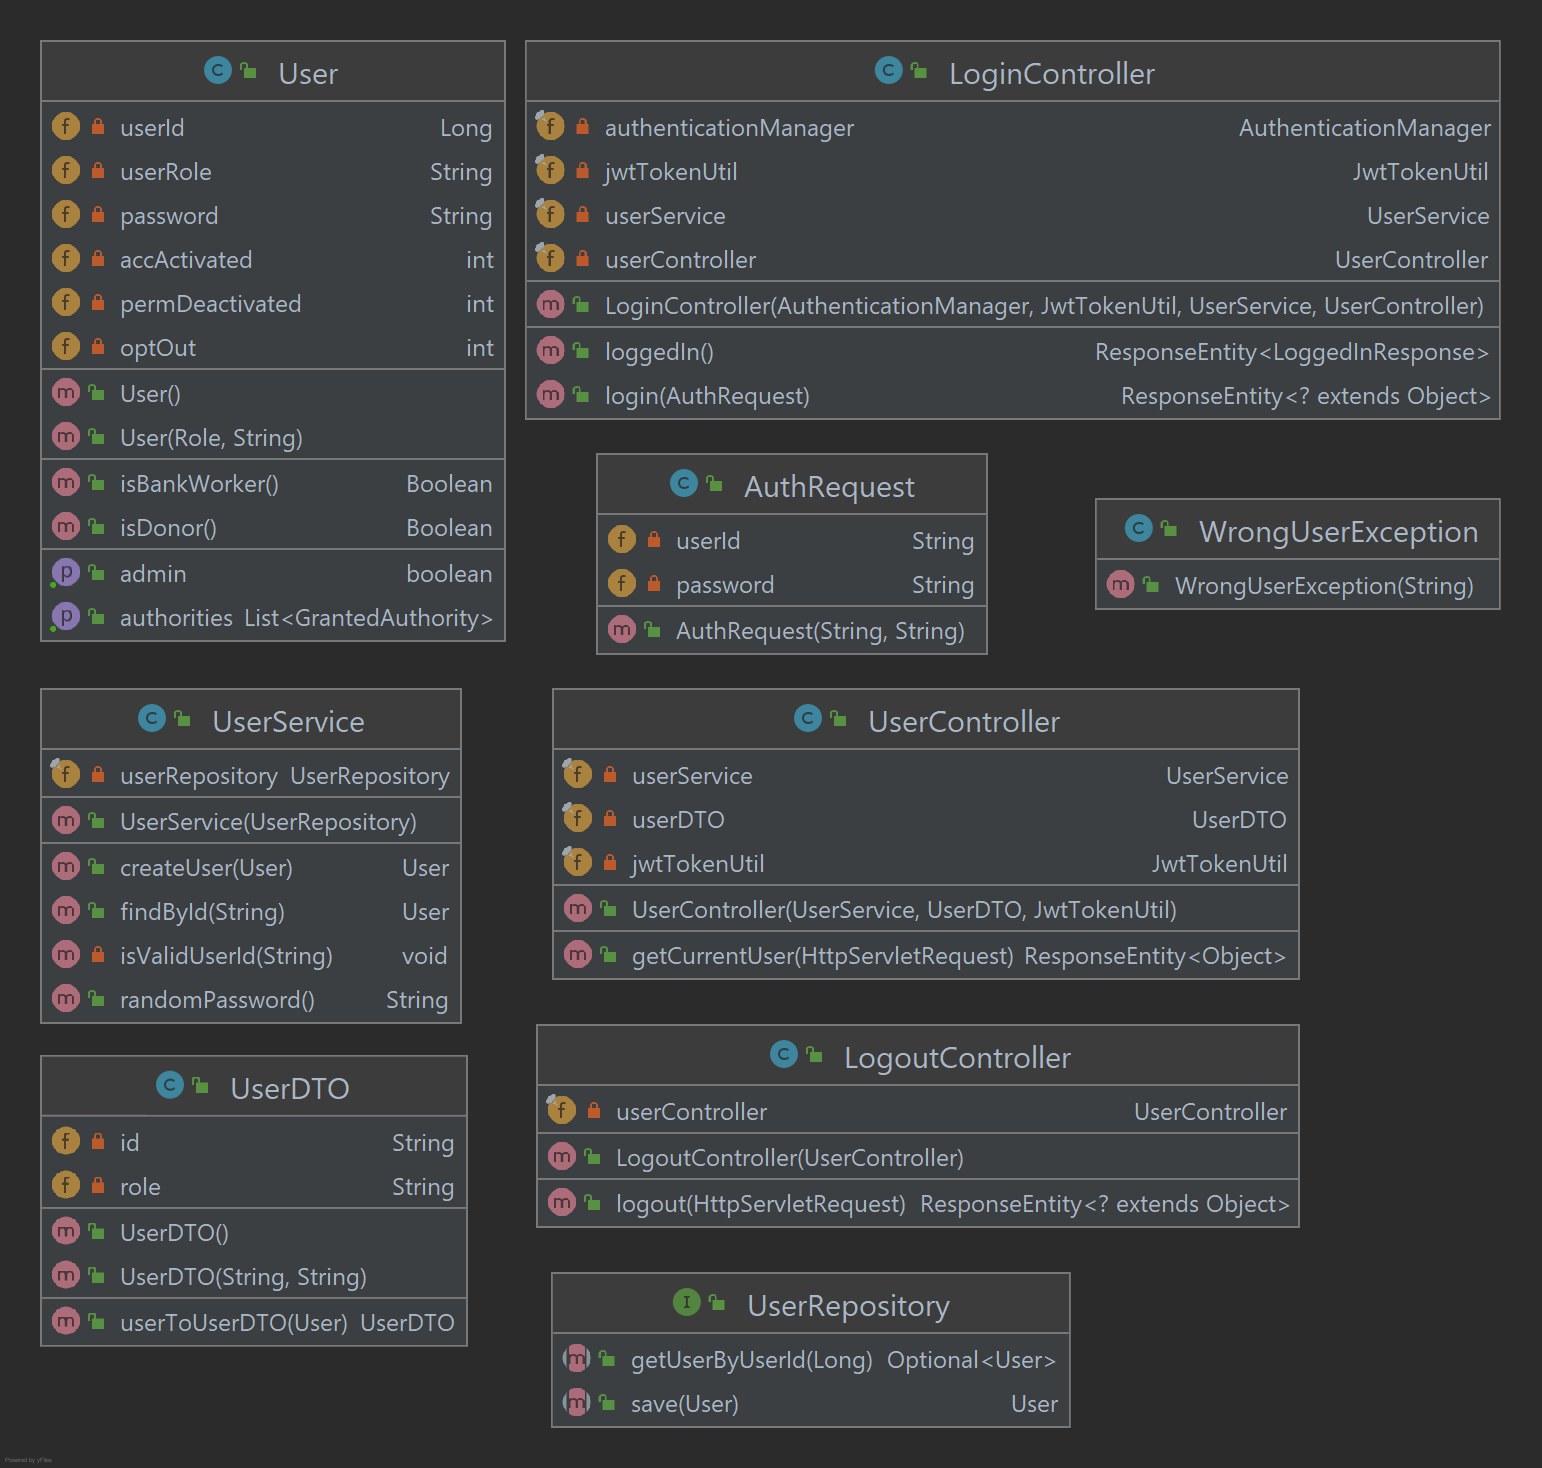
\includegraphics[scale=0.28]{slike/user.png}
        			\centering
        			\caption{Dijagram razreda vezanih za entitet Korisnik}
        			\label{fig:hztm-stranica}
        		\end{figure}

Entitetu Korisnik pripadaju klase LoginController i LogoutController.

LoginController je zadužen za ostvarivanje funkcionalnosti prijave. Lozinke se spremaju i provjeravaju u kodiranom obliku pomoću BCryptEncoder-a]. Dakle, koristi se sigurnosna shema Bearer Authentication.

LogoutController je zadužen za odjavu korisnika.

Entiteti Korisnik i Donor mogu uzrokovati iznimke ako se radi o krivom korisniku/donoru.

                \begin{figure}[H]
                    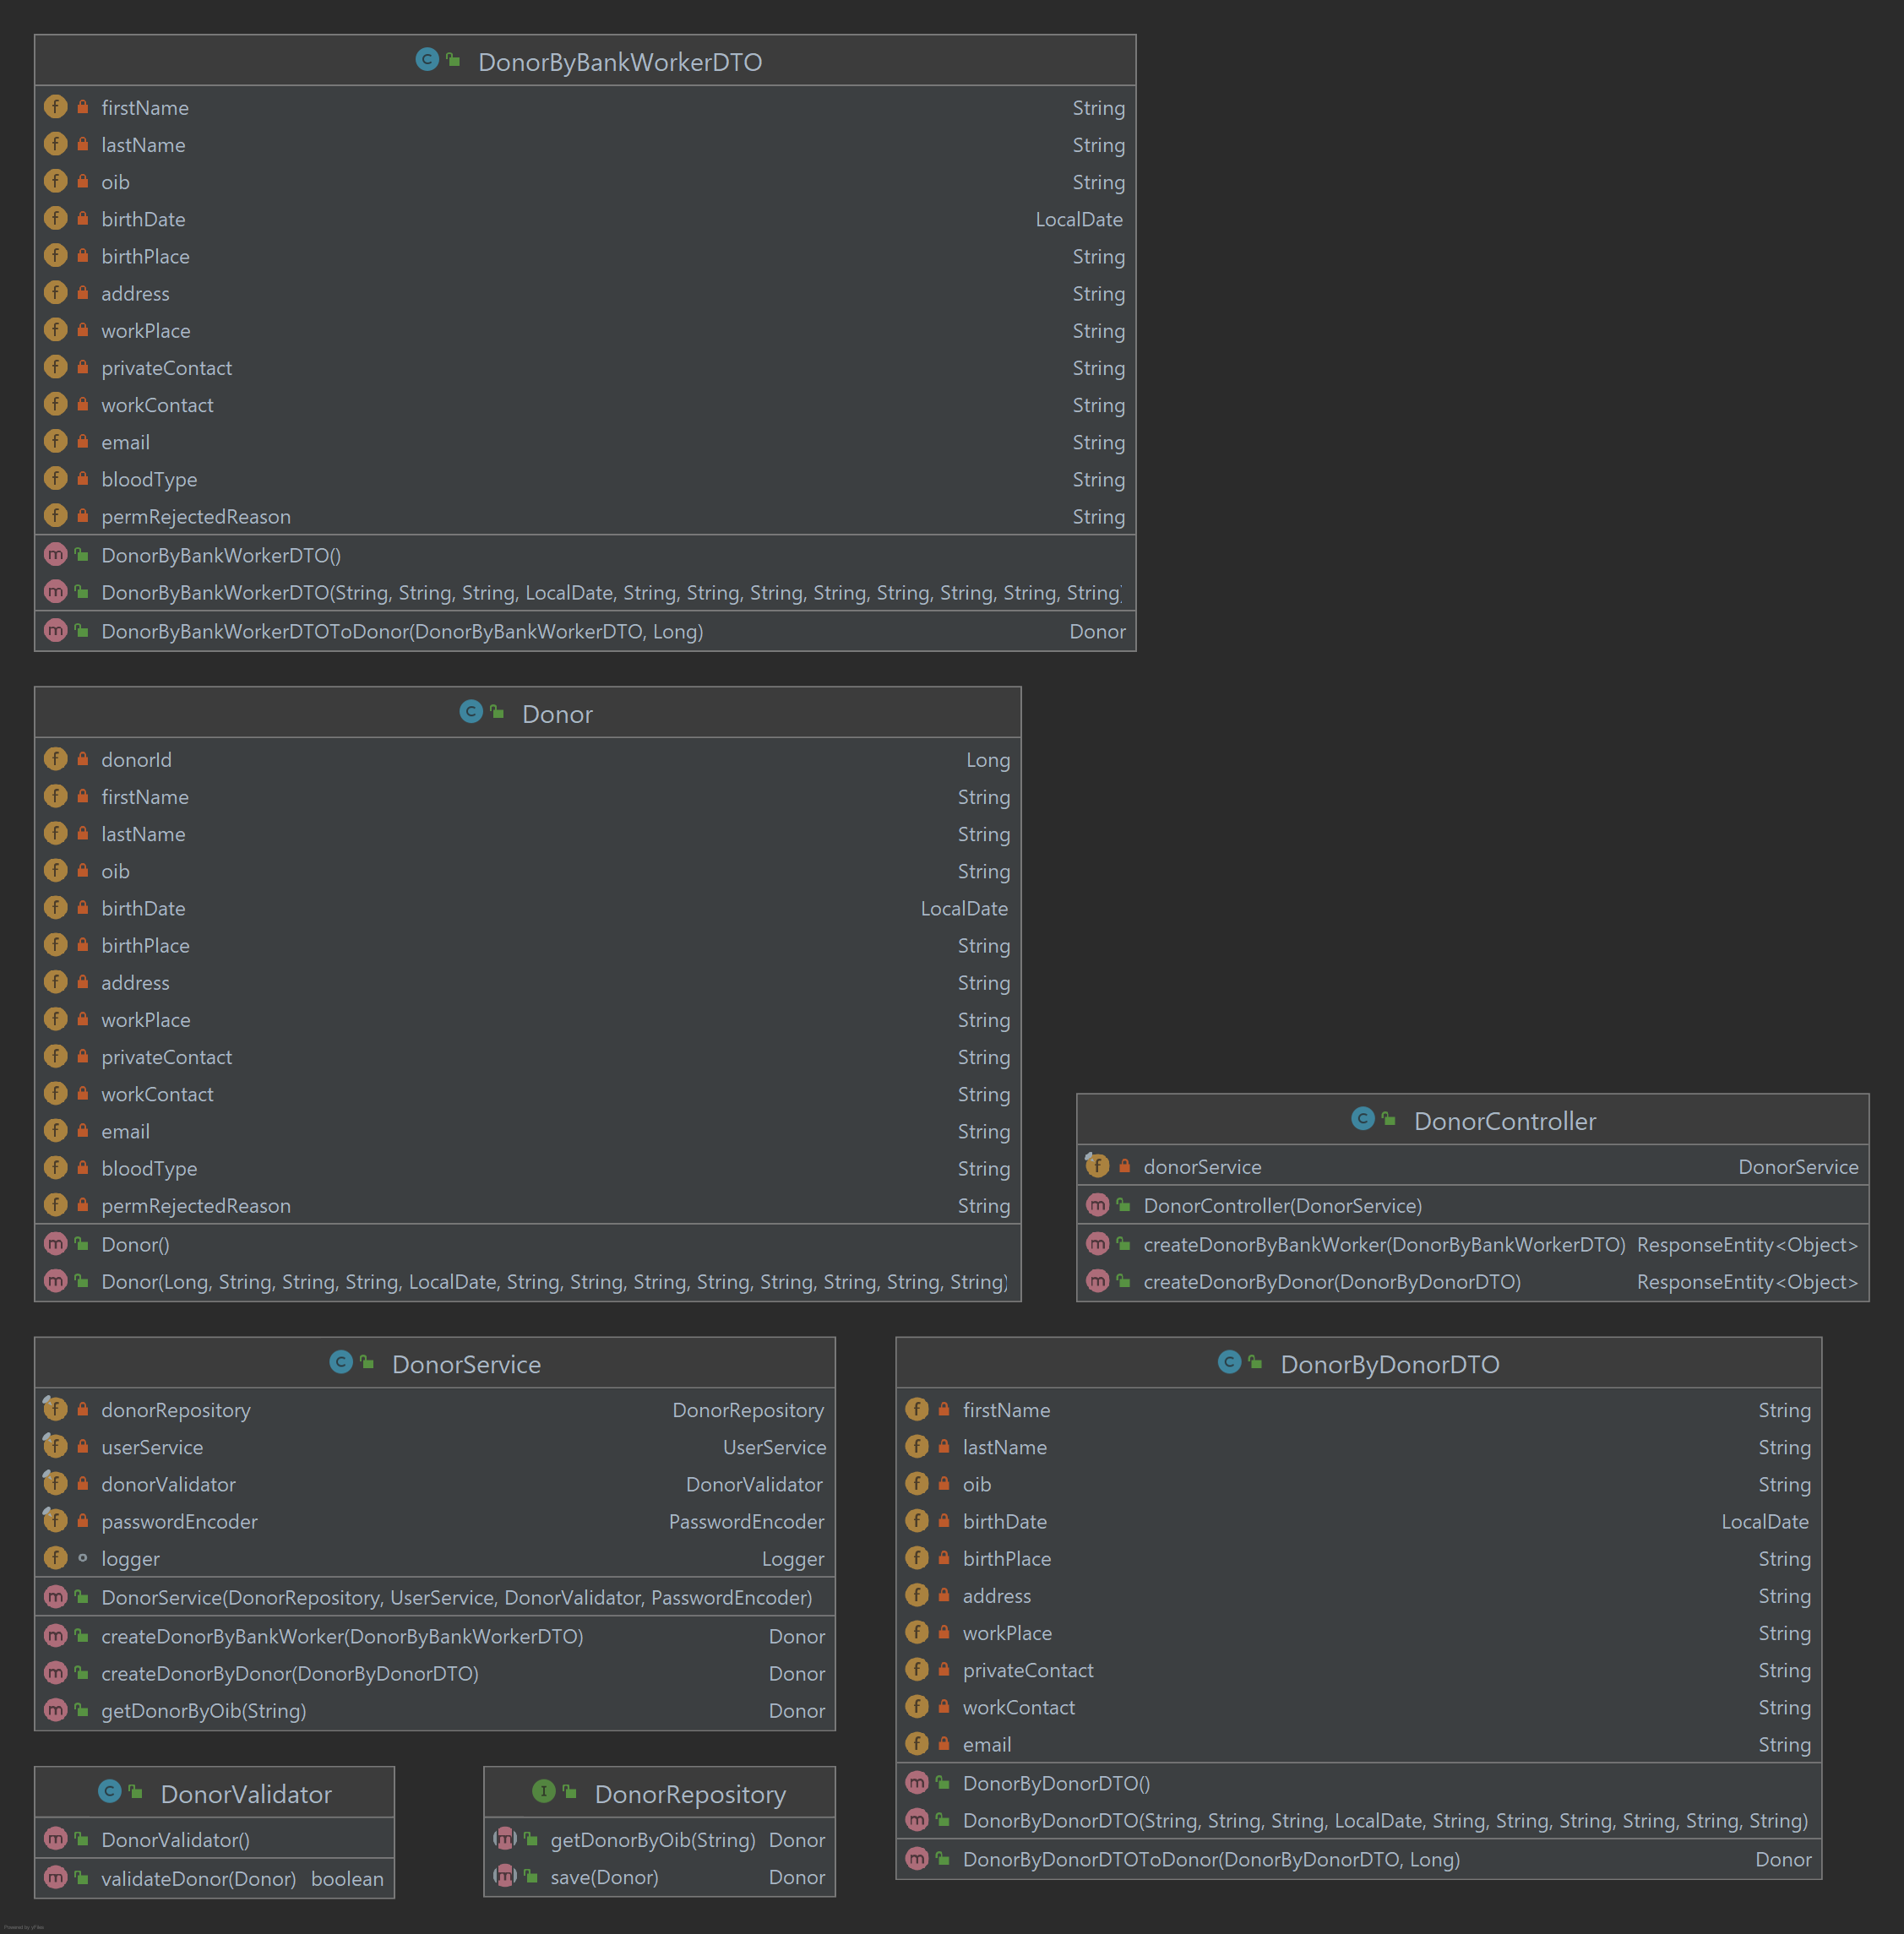
\includegraphics[scale=0.20]{slike/donor.png}
        			\centering
        			\caption{Dijagram razreda vezanih za entitet Donor}
        			\label{fig:hztm-stranica}
        		\end{figure}
        		
        		\begin{figure}[H]
                    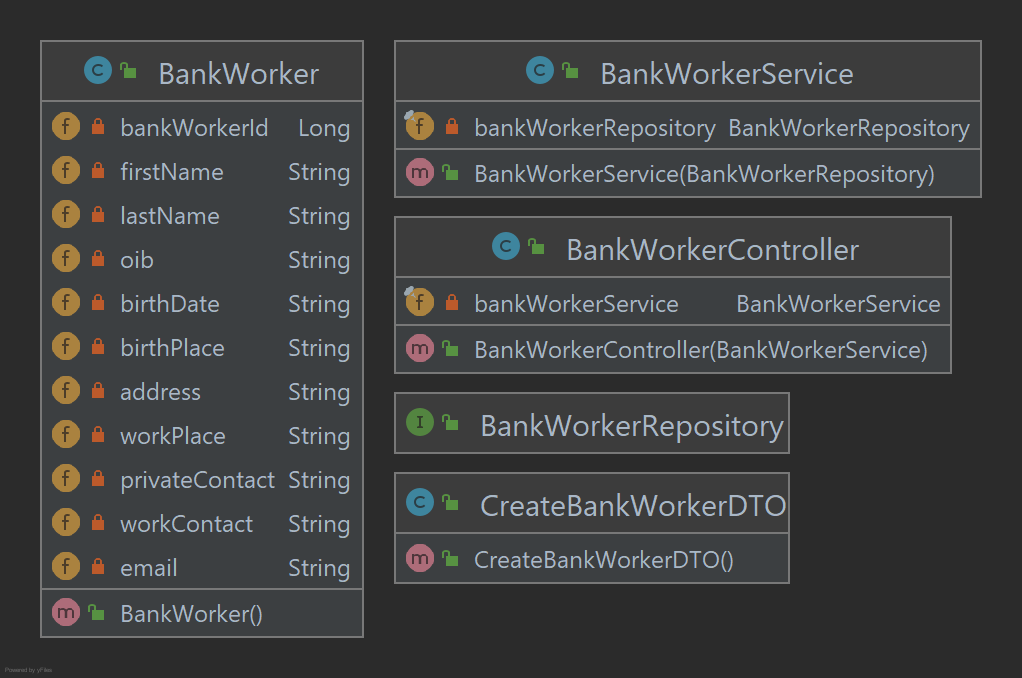
\includegraphics[scale=0.25]{slike/bankworker.png}
        			\centering
        			\caption{Dijagram razreda vezanih za entitet Djelatnika banke}
        			\label{fig:hztm-stranica}
        		\end{figure}
        		
        		\begin{figure}[H]
                    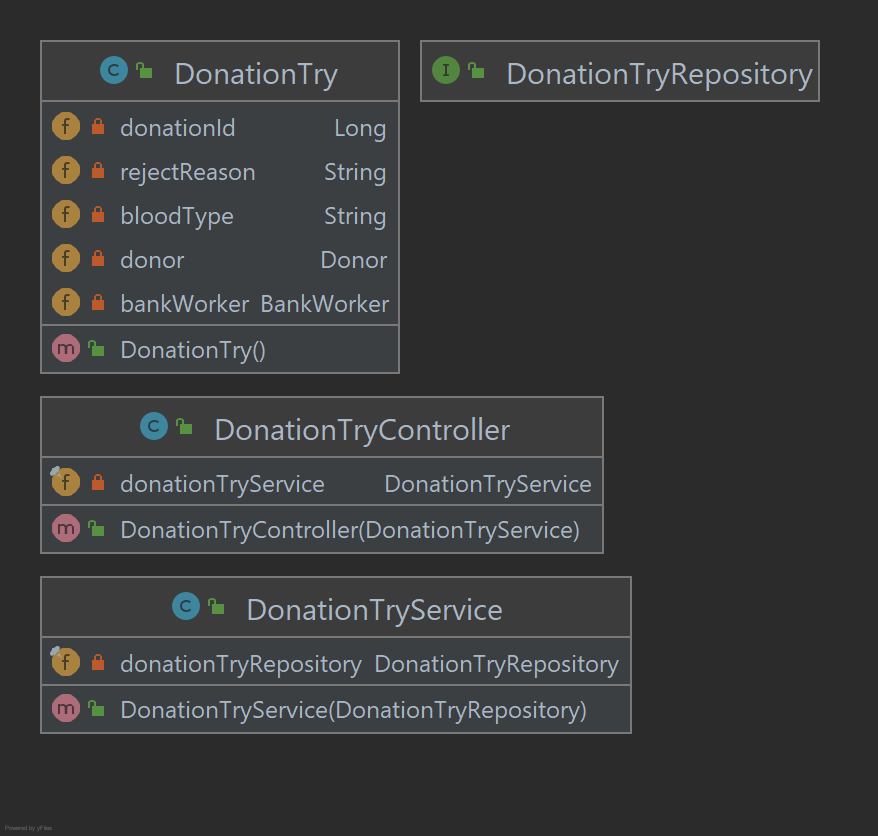
\includegraphics[scale=0.25]{slike/donationtry.png}
        			\centering
        			\caption{Dijagram razreda vezanih za entitet Pokušaj donacije}
        			\label{fig:hztm-stranica}
        		\end{figure}
        		
        		\begin{figure}[H]
                    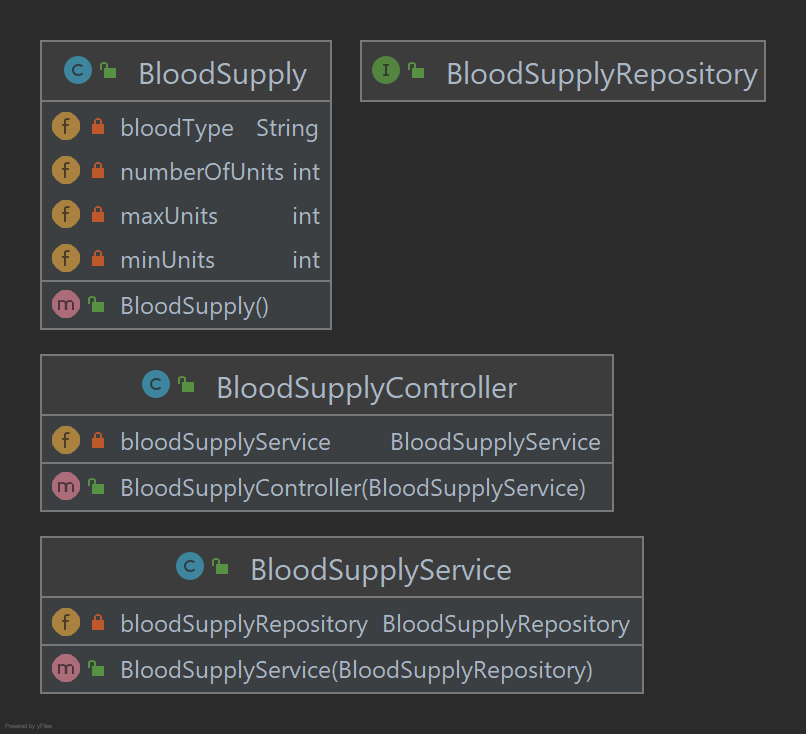
\includegraphics[scale=0.25]{slike/bloodsupply.png}
        			\centering
        			\caption{Dijagram razreda vezanih za entitet Zaliha krvi}
        			\label{fig:hztm-stranica}
        		\end{figure}
        		
        		\begin{figure}[H]
                    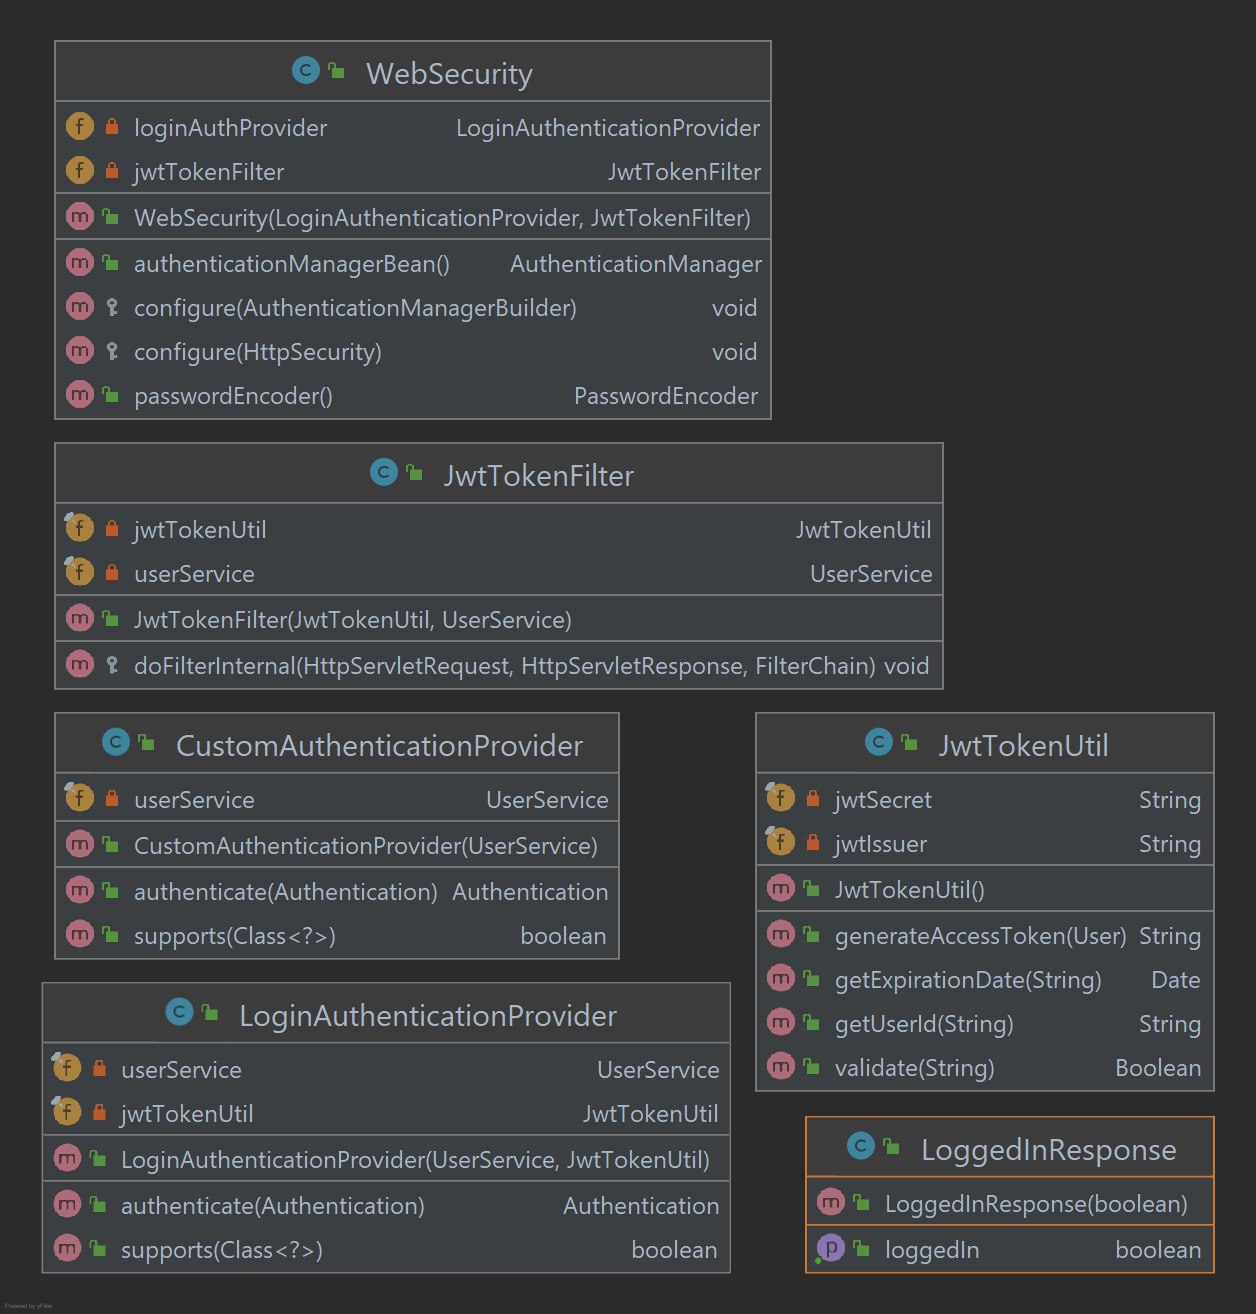
\includegraphics[scale=0.25]{slike/security.png}
        			\centering
        			\caption{Dijagram razreda vezanih za sigurnost i autentikaciju}
        			\label{fig:hztm-stranica}
        		\end{figure}
			
			Zadnja slika sadrži klase vezane za sigurnost i autentikaciju. Radi se o klasama koje pruža Spring. Koriste se Jwt Tokeni (iz biblioteke .jsonwebtoken.jjwt) koji osiguravaju identitet korisnika aplikacije.
			
%			\textbf{\textit{dio 2. revizije}}\\			
			
%			\textit{Prilikom druge predaje projekta dijagram razreda i opisi moraju odgovarati stvarnom stanju implementacije}
			
			
		    
		
		
%		\section{Dijagram stanja}
			
			
%			\textbf{\textit{dio 2. revizije}}\\
			
%			\textit{Potrebno je priložiti dijagram stanja i opisati ga. Dovoljan je jedan dijagram stanja koji prikazuje \textbf{značajan dio funkcionalnosti} sustava. Na primjer, stanja korisničkog sučelja i tijek korištenja neke ključne funkcionalnosti jesu značajan dio sustava, a registracija i prijava nisu. }
			
			

%		\section{Dijagram aktivnosti}
			
%			\textbf{\textit{dio 2. revizije}}\\
			
%			 \textit{Potrebno je priložiti dijagram aktivnosti s pripadajućim opisom. Dijagram aktivnosti treba prikazivati značajan dio sustava.}
			
%			\eject
%		\section{Dijagram komponenti}
		
%			\textbf{\textit{dio 2. revizije}}\\
		
%			 \textit{Potrebno je priložiti dijagram komponenti s pripadajućim opisom. Dijagram komponenti treba prikazivati strukturu cijele aplikacije.}